\documentclass[11pt]{article}
\usepackage[document]{ragged2e} % no indent line
\usepackage{amsmath} % math
\usepackage{hyperref} % url
\usepackage{mathtools} % norm
\DeclarePairedDelimiter{\norm}{\lVert}{\rVert}
\usepackage{listings} % show code
\usepackage{amssymb} % math symb
\usepackage[ruled,vlined]{algorithm2e} % algo
\usepackage{algorithmicx}

\title{TP de Calcul Numérique}
\author{Nicolas BOUTON}
\date{2020}

\begin{document}

\maketitle

\section{Exercice 1}

\subsubsection{Question 1}

Approximation de $T''$ au moyen d'un schéma centré d'ordre 2.\newline
\vspace{5mm}
Developpement limité : 

\begin{equation*}
  \begin{split}
    T(x_i + h) & = T(x_i) + h \left(\frac{\partial T}{\partial x} \right)_i + h^2 \left(\frac{\partial^2 T}{\partial x^2} \right)_i + O(h^2) \\
    T(x_i - h) & = T(x_i) - h \left(\frac{\partial T}{\partial x} \right)_i + h^2 \left(\frac{\partial^2 T}{\partial x^2} \right)_i + O(h^2)
  \end{split}
\end{equation*}

On somme et on inverse le signe :

\begin{equation*}
  \begin{split}
    - T(x_i + h) + 2 T(x_i) - T(x_i - h) = - h^2 \left(\frac{\partial^2 T}{\partial x^2} \right)_i + O(h^2) \\
    \frac{- T(x_i + h) + 2 T(x_i) - T(x_i - h)}{h^2} = - \left(\frac{\partial^2 T}{\partial x^2} \right)_i
  \end{split}
\end{equation*}

Donc
\begin{equation*}
  T'' = \frac{T(x + h) - 2 T(x) + T(x - h)}{h^2}
\end{equation*}

\subsubsection{Question 2}

On a :

\begin{equation*}
  - k \left( \frac{\partial^2 T}{\partial x^2} \right)_i = g_i, k > 0
\end{equation*}

On se permet de négligé k car c'est une constante dans nos prochain calcul:

\begin{equation*}
  \begin{split}
    - T(x_i + h) + 2 T(x_i) - T(x_i - h) = h^2 g_i
  \end{split}
\end{equation*}

On écrit le système d'équation : 

\begin{equation*}
  \begin{array}{ll}
    u_0 = T_0 & i = 0 \\
    - u_0 + 2 u_1 - u_2 = h^2 g_1 & i = 1\\
    ... & ... \\
    - u_{k-1} + 2 u_k - u_{k+1} = h^2 g_k & i = k\\
    ... & ... \\
    - u_{n-1} + 2 u_n - u_{n+1} = h^2 g_n & i = n\\
    u_n = T_n & i = n + 1 \\
  \end{array}
\end{equation*}

Avec les conditions aux bords on obtient :

\begin{equation*}
  \begin{array}{l}
    2 u_1 - u_2 = h^2 g_1 + T_0 \\
    - u_{n-1} + 2 u_n = h^2 g_n + T_n \\
  \end{array}
\end{equation*}

Donc on explicite le système linéaire $Au = g$ :

\begin{equation*}
  A = \left[
    \begin{array}{ccccccc}
      2 & -1 & 0 & - & - & - & 0 \\
      -1 & 2 & -1 & . &  &  & |  \\
      0 & -1 & . & . & . &  & |  \\
      | & . & . & . & . & . & |  \\
      | & & . & . & . & -1 & 0  \\
      | & & & . & -1 & 2 & -1  \\
      0 & - & - & - & 0 & -1 & 2 \\
    \end{array}
    \right]
\end{equation*}

\begin{equation*}
  u = \left[
    \begin{array}{c}
      T_1 \\
      | \\
      T_n \\
    \end{array}
    \right]
\end{equation*}

\begin{equation*}
  g = \left[
    \begin{array}{c}
      h^2 T_1 + T_0 \\
      h^2 T_2 \\
      | \\
      h^2 T_{n-1} \\
      h^2T_n + T_1\\
    \end{array}
    \right]
\end{equation*}

Comme il n'y a pas de source de chaleur, on a $\forall i \in [ 1, n
] : h^2 g_i = 0$

D'où $g = \left[
  \begin{array}{c}
    T_0 \\
    0 \\
    | \\
    0 \\
    T_1 \\
  \end{array}
  \right]$

Nous avons donc :

\begin{equation*}
  \left[
    \begin{array}{ccccccc}
      2 & -1 & 0 & - & - & - & 0 \\
      -1 & 2 & -1 & . &  &  & |  \\
      0 & -1 & . & . & . &  & |  \\
      | & . & . & . & . & . & |  \\
      | & & . & . & . & -1 & 0  \\
      | & & & . & -1 & 2 & -1  \\
      0 & - & - & - & 0 & -1 & 2 \\
    \end{array}
    \right]
  \left[
    \begin{array}{c}
      T_1 \\
      T_2 \\
      | \\
      | \\
      | \\
      T_{n - 1} \\
      T_n \\
    \end{array}
    \right]
  =
  \left[
  \begin{array}{c}
    T_0 \\
    0 \\
    | \\
    | \\
    | \\
    0 \\
    T_1 \\
  \end{array}
  \right]
\end{equation*}

Et la solution analytique qui se déguage est : 

$$ T(x) = T_0 + x (T_1 - T_0) $$

\section{Exercice 2}
\subsection{Arch}
\subsubsection{Bibliothèque}

Pour l'intallation des bibliothèque \textbf{cblas} et \textbf{lapacke}
:
\newline
\$ sudo pacman -S cblas lapacke

\subsubsection{Makefile}

Il faut modifier la ligne qui link les librairie en linkant la
bibliothèque \textbf{cblas}:

\# \\
\# -- librairies \\
LIBS=-llapacke -lcblas -lm \\

\section{Exercice 3}
\subsection{Question 1}

Les matrices pour utiliser \textbf{BLAS} et \textbf{LAPACK} en \textbf{C} sont allouées
et déclarées de la même manière que les tableaux en \textbf{C}. Mais elles
doivent être stockées dans l'un des formats suivant :

\begin{itemize}
\item stockage conventionnel en 2 dimension (ex: int tab[10][10])
\item stockage compact pour les matrices symétrique, hermitienne et
  triangulaire (stockage dans un tableau à 1 dimension des éléments
  de la matrice supérieur ou inférieur)
\item stockage bandes pour les matrices à bandes (cad que les
  diagonales autour de la diagonale principale contiennent la
  plupart des NNZ) (GB et GE)
\item utilisation de 2 ou 3 tableaux à 1 dimension pour stocker les
  matrices bidiagonale et tridiagonale respectivement
\end{itemize}

source : \url{http://performance.netlib.org/lapack/lug/node121}

\subsection{Question 2}

\begin{itemize}
\item Les constantes LAPACK\_ROW\_MAJOR et LAPACK\_COL\_MAJOR
  signifie la priorité ligne ou colonne respectivement de la
  représentation de la matrice.
\item Effectivement, cet argument sert si on utilise un stockage
  par priorité ligne ou colonne car il faut préciser si on a utilisé
  une priorité ligne ou colonne pour stocker la matrice pour pouvoir
  faire les bons calculs.
\end{itemize}

\subsection{Question 3}
   
La \textbf{leading dimension} permet de savoir qu'elle élément correspond
à la prochaine colonne ou la prochaine ligne suivant le stockage
colonne ou ligne respectivement.

\begin{itemize}
\item Si on choisis un stockage priorité ligne, alors la \textbf{leading dimension}
  correspond au nombre d'élément d'une ligne pour
  pouvoir accéder à la ligne suivante.
\item Si on choisis un stockage priorité colonne, alors la \textbf{leading dimension}
  correspond au nombre d'élément d'une colonne pour
  pouvoir accéder à la colonne suivante.
\end{itemize}

\subsection{Question 4}
\subsubsection{Résumé}

La fonction LAPACKE\_dgbsv permet de calculer le résultat d'un
système linéaire du type $A * X = B$, avec \textbf{X} l'inconnu, \textbf{A} une
matrice et \textbf{B} le second membre, où \textbf{X} et \textbf{B} peuvent être des
vecteurs ou des matrices.

\subsubsection{Argument}

Elle prend en argument la dimension de la matrice, le nombre du
sous-diagonnale ainsi que de sur-diagonnale, la leading dimension de
\textbf{A} et de \textbf{B}, le nombre de colonne de \textbf{B} ainsi
que tableau d'entier pour stoker les indices de permutation.

\subsubsection{Implémentation}

Cette fonction implémente une décomposition \textbf{LU} à pivot partiel et
la méthode de dessente et de remonté.

\subsubsection{Note importante}

Pour la factorisation \textbf{LU}, la fonction a besoin d'un vecteur de
travail ou il stockera les pivots. Suivant le stockage choisis on
rajoutera une ligne ou une colonne avant de stocker notre matrice
car le vecteur doit apparaître en premier.

\subsubsection{Sources}

\url{http://www.math.utah.edu/software/lapack/lapack-d/dgbsv.html}
   
\subsection{Question 5}
A titre comparatif nous prendrons une matrice de taille 10 x 10.

\subsubsection{Stockage priorité colonne}

\begin{equation*}
  \begin{array}{rrrr}
    0.000000 &	0.000000  &	2.000000 &	-1.000000	\\
    0.000000 &	-1.000000 &	2.000000 &	-1.000000	\\
    0.000000 &	-1.000000 &	2.000000 &	-1.000000	\\
    0.000000 &	-1.000000 &	2.000000 &	-1.000000	\\
    0.000000 &	-1.000000 &	2.000000 &	-1.000000	\\
    0.000000 &	-1.000000 &	2.000000 &	-1.000000	\\
    0.000000 &	-1.000000 &	2.000000 &	-1.000000	\\
    0.000000 &	-1.000000 &	2.000000 &	-1.000000	\\
    0.000000 &	-1.000000 &	2.000000 &	-1.000000	\\
    0.000000 &	-1.000000 &	2.000000 &	0.000000	\\
  \end{array}
\end{equation*}

\subsubsection{Stockage priorité ligne}

\begin{equation*}
  \begin{array}{rrrrrrrrrr}
    0.000 &	0.000 &	0.000 &	0.000 &
    0.000 &	0.000 &	0.000 &	0.000 &
    0.000 &	0.000 \\	
    0.000 &	-1.000 &	-1.000 &	-1.000 &
    -1.000 &	-1.000 &	-1.000 &	-1.000 &
    -1.000 &	-1.000 \\
    2.000 &	2.000 &	2.000 &	2.000 &
    2.000 &	2.000 &	2.000 &	2.000 &
    2.000 &	2.000 \\	
    -1.000 &	-1.000 &	-1.000 &	-1.000 &
    -1.000 &	-1.000 &	-1.000 &	-1.000 &
    -1.000 &	0.000 \\
  \end{array}
\end{equation*}

Pour que le tableau soit affichable nous avons dû enlever les 3
derniers 0 de la sortie, mais cela ne change pas le résultat.

\subsubsection{Remarques}

Nous pouvons apercevoir que nous avons le bon résultat, étant donné
que la première ligne qui réservé à \textbf{BlAS} pour son vecteur de
travail est constitué de zéro ainsi que le premier élément de la
diagonale supérieur et le dernier élément de le diagonale
inférieur.\newline

De plus pour vérifier le résultat il suffit de calculer la transposé
de l'une des matrices et la comparé à la deuxième car elles doivent
être égales. Ici la transposé d'une des 2 matrices est égales à la
deuxième.

\section{Exercice 5}

\subsection{Question 1}

\subsubsection{Equation}

La fonction \textbf{cblas\_dgbmv} permet de calculer l'équation
suivante :

\begin{equation*}
y = \alpha * A * x + \beta * y
\end{equation*}

Dans notre cas on a l'équation suivante :

\begin{equation*}
A * u = b
\end{equation*}

Qu'on peut écrire avec les notations de l'équation juste au dessus :

\begin{equation*}
A * y = x
\end{equation*}

Avec la question précédente on a calculer y. On peut donc tester la
fonction sur l'équation suivante :

\begin{equation*}
x = 1 * A * y + 0 * x
\end{equation*}

\subsubsection{Argument}

La fonction \textbf{cblas\_dgbmv} prends à peut près les mêmes
paramètres que \textbf{LAPACKE\_dgbsv} plus les coefficient $\alpha$
et $beta$, le nombre de ligne et de colonne de la matrice en format
classic ainsi qu'un paramètre qui indique si la matrice est une
transposé ou non.\newline

La fonction prend comme précondition que y et x soit des vecteurs.

\subsubsection{Note importante}

Contrairement à la fonction \textbf{LAPACKE\_dgbsv}, la fonction
\textbf{cblas\_dgbmv} n'attend pas à ce qu'on lui laisse un vecteur au
début de la matrice.

\subsection{Question 2}

Comme méthode de validation, nous proposons de calculé l'erreur
relative suivante.\newline

Etant donné que nous calculons l'équation suivante :

\begin{equation*}
b = A * u
\end{equation*}

Nous allons calculer l'erreur relative suivante :

\begin{equation*}
relres = \frac{\norm{EX\_SOL - B}}{\norm{B}}
\end{equation*}

où \textbf{B} est en fait le résultat calculé et \textbf{EX\_SOL} la
solution exacte.\newline
Le résultat exacte de \textbf{B} est stocké dans le fichier \textbf{B.dat}.

\subsubsection{Priorité Ligne}

Le résultat est stocké dans le fichier \textbf{Y\_row.dat}.\newline

\begin{lstlisting}
--------- Poisson 1D ---------


 INFO DGBSV = 0

The relative residual error is relres = 1.764638e-16

 DGBSV :

The relative residual error is relres = 5.102197e-16


--------- End -----------
\end{lstlisting}

Pour la priorité ligne il faut stocké les lignes en colonne et mettre
comme leading dimension la leading dimension des colonnes donc
conformément au code FORTRAN de BLAS qui stipule que la transposé de
la matrice est calculé et utilisé à la place de la matrice d'entré si
jamais on entre l'argument \textbf{CblasNoTrans}.

\subsubsection{Priorité Colonne}

Le résultat est stocké dans le fichier \textbf{Y\_col.dat}.

\begin{lstlisting}
--------- Poisson 1D ---------


 INFO DGBSV = 0

The relative residual error is relres = 1.764638e-16

 DGBSV :

The relative residual error is relres = 5.102197e-16


--------- End -----------
\end{lstlisting}

\subsubsection{Explication}

L'erreur relative de la fonction \textbf{cblas\_dgbmv} est un peut
plus élevé que l'erreur relative de la fonction
\textbf{LAPACKE\_dgbsv} qui peut être expliqué par le fait que le bit
de signe ne change pas et nous nous retrouvons avec des zéro négatif
au lieu de positif mais l'erreur reste acceptable car il est de
l'ordre de la précision machine.

\subsubsection{Conclusion}

Nous pouvons donc validé l'appelle a blas pour la priorité colonne
mais pas pour la priorité ligne pour le moment.

\section{Exercice 5}

\subsection{Question 1}

\subsubsection{Implémentation scilab}

Voir le premier rapport.

\subsubsection{Implémentation C}

\subsubsection{Code}

Le code est séparé en deux fichier, un contenant le code des fonction
qui se trouve dans \textbf{src/lib\_lu.c}, et un fichier qui contient
le code de test qui est dans \textbf{src/tp2\_facto\_lu.c}.\newline

Pour compiler : \$ make tp2facto\_lu\newline
Pour executer : \$ make run\_tp2facto\_lu\newline

\subsubsection{Explication}

Nous avons effectuer une résolution d'un sytème linéaire tel que $A *
x = b$ ou bien même $LU * x = b $ grâce à une factorisation
LU.\newline
\vspace{5mm}
Puis avec une méthode de dessente : $ L * y = b $.\newline
Puis avex une méthode de remonté : $ U * x = y $.\newline
\vspace{5mm}
Pour cela nous avons dû utiliser 1 matrice A et deux vecteurs X et B
où A est une matrice tridiagonnale stocké en format général bandes 
priorité colonne de taille $3 * la$ (où \textbf{la} est la leading dimension de
A), X un vecteur de taille \textbf{la} ainsi que B un vecteur de
taille \textbf{la}.\newline
\vspace{5mm}
Et nous effecturons les opérations suivantes :

\begin{equation*}
  \left\{
  \begin{array}{l}
    A = LU(A) \\
    L * X = B \\
    U * B = X \\
  \end{array}
  \right.
\end{equation*}

\begin{itemize}
\item on effectue la factorisation LU de A que l'on stocke dans A
\item on effectue la méthode de dessente sur L et B et l'on stocke le
  résultat dans X
\item on effectue la méthode de remonté sur U et X et l'on stocke le
  résultat dans B
\item le résultat est bien dans le second membre c'est-à-dire B
\end{itemize}

\subsection{Question 2}

Pour la méthode de validation, nous allons calculer l'erreur relative
avant et s'assurer que l'erreur est proche de la précision machine.

\subsubsection{Calcul}

\begin{equation*}
relres = \frac{\norm{EX\_SOL - B}}{\norm{B}}
\end{equation*}

où EX\_SOL est la solution exacte et B la solution calculé.

\subsubsection{Résultat}

\begin{lstlisting}
--------- Facto LU ---------

The relative residual error is relres = 1.764638e-16

----------- End ------------
\end{lstlisting}

\subsubsection{Conclusion}

Le résultat de l'erreur est bien proche de la précision machine donc
on peut valider notre algorithme et notre implémentation.

\subsubsection{Comparaison avec cblas\_dgbmv}

L'erreur relative pour les deux calculs sont les mêmes, en effet la
fonction de BLAS fait les mêmes que ce que l'ont a fait pour le
cas particulier d'une matrice tridiagonnale mais sur des matices avec
plus ou moins de diagonales. Il faudrai étudier le temps que prends les
deux méthodes pour pouvoir mieux les comparer.

\section{Exercice 6}

\subsection{Question 1}

On ajoute une nombre d'itération maximale pour éviter une boucle
infini à cause de l'une des raisons suivantes :

\begin{itemize}
\item la solution ne converge pas
\item la solution converge mais met très longtemps à convergé et nous
  voulons limité le temps
\end{itemize}

\subsubsection{Jacobi}

\begin{algorithm} [H]
  \SetAlgoLined
  \KwData{$A \in \mathbb{R}^{n \cdot n}$, $b \in \mathbb{R}^{n}$,
    $max\_count, \epsilon \in \mathbb{R}$}
  \KwResult{$x \in \mathbb{R}^{n}$, $count, relres \in \mathbb{R}$, $resvec \in
    \mathbb{R}^{n}$}
  
  \For{$i = 1:n$} {
    $D(i,i) = \frac{1}{A(i, i)}$ \Comment{Init. matrice D}
  }

  count = 0 \Comment{Init. compteur}

  x = zeros(n) \Comment{Init. vecteur résultat à 0}

  normb = norm(b) \Comment{Init. norme de b}

  r = b - A * x \Comment{Init. résidu}

  relres = norm(r) / normb \Comment{Init. erreur relative}

  \While{$relres > \epsilon$ and $count < max\_count$}{

    x = x + D * r \Comment{Calcul de Richardson}

    r = b - A * x \Comment{Calcul du résidu}
    
    relres = norm(r) / normb \Comment{Calcul de l'erreur relative}
    
    resvec(count) = relres \Comment{Sauv. vecteur}

    count = count + 1; \Comment{Inc. compteur}
  }

  \caption{Applique le méthode de Jacobi}
\end{algorithm}

\subsubsection{Gauss Seidel}

\begin{algorithm} [H]
  \SetAlgoLined
  \KwData{$A \in \mathbb{R}^{n \cdot n}$, $b \in \mathbb{R}^{n}$,
    $max\_count, \epsilon \in \mathbb{R}$}
  \KwResult{$x \in \mathbb{R}^{n}$, $count, relres \in \mathbb{R}$, $resvec \in
    \mathbb{R}^{n}$}
  
  \For{i = 1:n} {
    D(i, i) = A(i, i) \Comment{Init. matrice D}
  }

  \For{i = 2:n} {
    E(i, i - 1) = - A(i, i - 1) \Comment{Init. matrice E}
  }

  DE = inverse(D - E) \Comment{Inverse (D - E)}

  count = 0 \Comment{Init. compteur}

  x = zeros(n) \Comment{Init. vecteur résultat à 0}

  normb = norm(b) \Comment{Init. norme de b}

  r = b - A * x \Comment{Init. résidu}

  relres = norm(r) / normb \Comment{Init. erreur relative}

  \While{$\norm{r} > \epsilon$ and $count < max\_count$}{

    x = x + DE * r \Comment{Calcul de Richardson}

    r = b - A * x \Comment{Calcul du résidu}

    relres = norm(r) / normb \Comment{Calcul erreur relative}

    resvec(i) = relres \Comment{Stocke erreur relative}
    
    count = count + 1 \Comment{Inc. compteur}
  }

  \caption{Applique le méthode de Gauss Seidel}
\end{algorithm}

\subsection{Question 2}

Pour nos deux algorithme, nous voyons que la complexité en temps ne
peux pas être explicite car tout dépend de l'erreur. D'après le cours
on était réduit à la formule ci dessous :\newline
\vspace{5mm}
Pour Jacobi :

\begin{equation*}
  k = - \frac{p}{2 * log(cos(\pi * h))}
\end{equation*}

Pour Gauss Seidel :

\begin{equation*}
  k = - \frac{p}{log(cos(\pi * h))}
\end{equation*}

avec

\begin{itemize}
\item k le nombre d'itération
\item p le nombre de chiffre significatif de l'erreur
\item h un entier quelconque
\end{itemize}

\subsubsection{Jacobi}

\underline{Complexité :}

\begin{itemize}
\item en temps : indéterminé (dépend des paramètre d'entré)
\item en temps d'une itération : $O(2n^2 + 2n)$ (2 produit \textbf{matrice x
  matrice} et 2 adition \textbf{vecteur x vecteur})
\item en espace : $O(2n^2 + 3n)$ (2 matrice + 3 vecteur)
\end{itemize}

\subsubsection{Gauss Seidel}

\underline{Complexité :}

\begin{itemize}
\item en temps : indéterminé (dépend des paramètre d'entré)
\item en temps d'une itération : $O(2n^2 + 2n)$ (2 produit \textbf{matrice x
  matrice} et 2 adition \textbf{vecteur x vecteur})
\item en espace : $O(4n^2 + 3n)$ (4 matrice + 3 vecteur)
\end{itemize}

Pour améliorer nos algorithmes d'un point de vu mémoire ainsi qu'en
tant on pourrai transformé les matrices en format général bandes, on
pourrai facilement calculé l'inverse des matrices pour les 2 méthodes
car ici on est dans un cas particuliers des matrices
tridiagonnales. Et dans la boucle \textbf{do...while} on fera appelle
à la fonction de blas \textbf{dgvsv} pour nos 2 opérations car se sont
en faites des systèmes linéaires. Il faudra juste multiplié par $-1$
le produit \textbf{matrice x vecteur} de la deuxième opération pour
les 2 méthodes.

\subsubsection{Amélioration pour Jacobi}

Pour l'équation de la chaleur, sur la diagonale de la matrice A on a
les même valeur et donc l'inverse sera aussi la même valeur pour toute
la diagonale donc on peut réduire le produit \textbf{matrice x
  vecteur} ($D * r$) en produit \textbf{scalaire x vecteur}.\newline
\vspace{5mm}
\begin{algorithm} [H]
  \SetAlgoLined
  \KwData{$A \in \mathbb{R}^{n \cdot n}$, $b \in \mathbb{R}^{n}$,
    $max\_count, \epsilon \in \mathbb{R}$}
  \KwResult{$x \in \mathbb{R}^{n}$, $count, relres \in \mathbb{R}$, $resvec \in
    \mathbb{R}^{n}$}

  D = 1 / 2 \Comment{Simplification}

  count = 0 \Comment{Init. compteur}

  x = zeros(n) \Comment{Init. vecteur résultat à 0}

  normb = norm(b) \Comment{Init. norme de b}

  r = b - A * x \Comment{Init. résidu}

  relres = norm(r) / normb \Comment{Init. erreur relative}

  \While{$relres > \epsilon$ and $count < max\_count$}{
    x = x + D * r \Comment{Calcul de Richardson}

    r = b - A * x \Comment{Calcul du résidu}

    relres = norm(r) / normb \Comment{Calcul erreur relative}

    resvec(i) = relres \Comment{Stocke erreur relative}
    
    count = count + 1 \Comment {Inc. compteur}
  }

  \caption{Applique le méthode de Jacobi}
\end{algorithm}
\vspace{5mm}
Ce qui nous conduit au complexité suivantes :

\begin{itemize}
\item en temps : indéterminé (dépend des paramètre d'entré)
\item en temps d'une itération : $O(n^2 + 3n)$ (1 produit \textbf{matrice x
  matrice}, 1 produit \textbf{scalaire x vecteur} et 2 adition
  \textbf{vecteur x vecteur})
\item en espace : $O(n^2 + 3n)$ (1 matrice + 3 vecteur)
\end{itemize}

\subsection{Question 3}

Pour $n = 3$ on obtient le nombre d'itération suivante :

\begin{center}
  \begin{tabular}{|r|r|r|}
    \hline
    $\epsilon$ & jacobi & gauss seidel \\ \hline
    $10^{-1}$ & 9 & 5 \\ \hline
    $10^{-2}$ & 16 & 8 \\ \hline
    $10^{-3}$ & 22 & 12 \\ \hline
    $10^{-4}$ & 29 & 15 \\ \hline
    $10^{-5}$ & 36 & 18 \\ \hline
    $10^{-6}$ & 42 & 22 \\ \hline
    $10^{-7}$ & 49 & 25 \\ \hline
    $10^{-8}$ & 56 & 28 \\ \hline
  \end{tabular}
\end{center}

Ce qui confirme l'approximation analytique qui dit que \textbf{Jacobi}
à besoin de 2 fois plus d'itération que \textbf{Gauss Seidel} pour
convergé.

\subsection{Question 4}

\underline{librairie :} voir dans le fichier
\textbf{src/iterative.sci}\newline
\underline{Explication :}\newline
Simple implémentation qui respecte les algorithmes ci-dessus, rien à
dire de spécial.\newline
\vspace{5mm}
\underline{script test :} voir dans le fichier
\textbf{src/tp2\_iterative.sci}\newline
\underline{Explication :}\newline
Il y a deux boucles, une qui vari la taille de la matrice et une qui
varie l'erreur souhaité pour voir l'évolution du nombre d'itération.

\subsubsection{Varié la taille de la matrice}

Ici un graphe qui montre l'évolution du nombre d'itération nécessaire
en fonction de la taille de la matrice A afin d'atteindre la
convergence pour une erreur de $10^{-8}$.

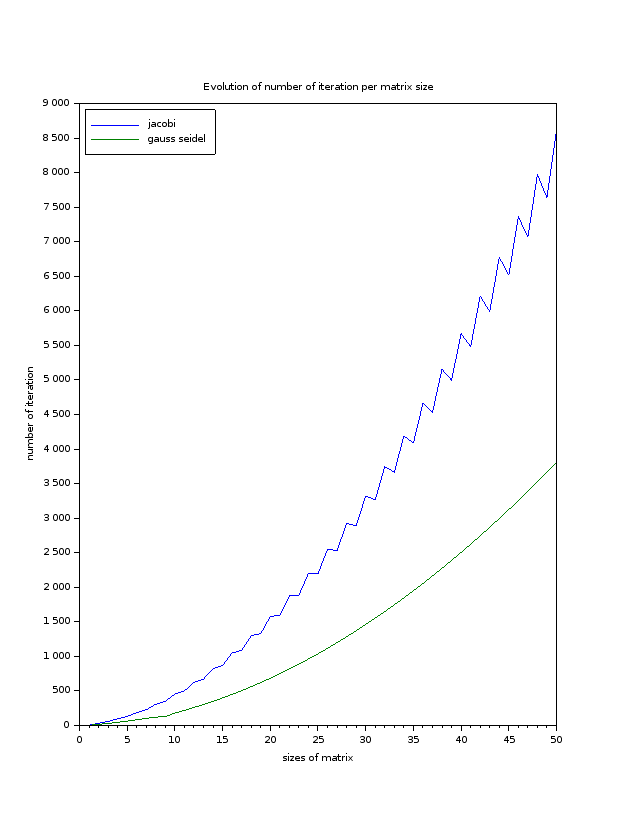
\includegraphics[scale=0.5]{img/number_of_iteration.png}

Nous pouvons appercevoir que le nombre d'itération évolue de manière
\textbf{quadratique} ce qui est normal car nous stockons les matrices en format
classique et donc elle augmente le nombre d'élément de façon
quadratique et c'est donc plus difficiles d'arrivé à convergeance.\newline

\vspace{5mm}

Nous voyons aussi que pour jacobi le nombre d'itération varie celon la
parité de la taille de la matrice, en effet lorsque la taille est pair
elle coute moins d'itération que ses voisins impair.\newline

\vspace{5mm}
\underline{Erreur relative avant :}\newline
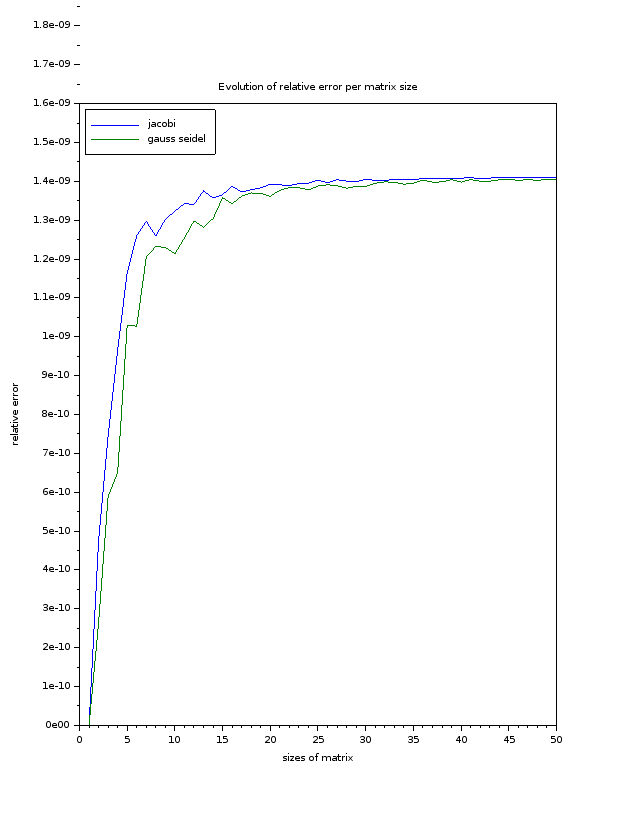
\includegraphics[scale=0.5]{img/number_of_iteration_relres.png}

Nous pouvons voir que l'erreur avant est très bonne étant donné
qu'on a fixé l'erreur machine à $10^{-16}$ et nous avons des erreurs
supérieur à celle-ci pour des matrices de taille \textbf{50 x 50}
maximum.

\subsubsection{Varié l'erreur souhaité}

Ici un graphe qui montre l'évolution du nombre d'itération nécessaire
en fonction de l'erreur souhaité afin d'atteindre la convergence pour
une taille de matrice $n = 10$, soit une matrice 10 x 10.

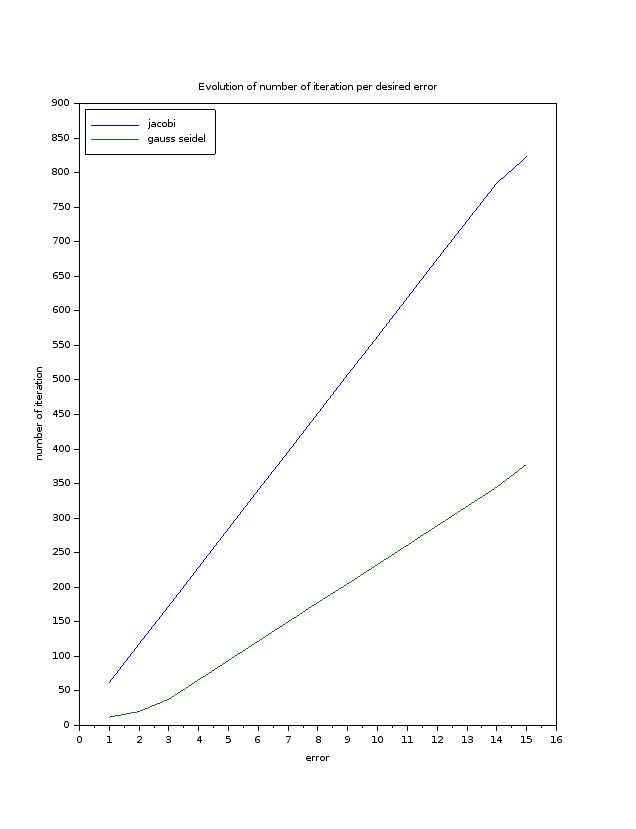
\includegraphics[scale=0.5]{img/error.png}

Nous pouvons apercevoir que lorsque l'on diminu l'erreur souhaité le
nombre d'itération évolue de manière \textbf{linéaire} car le fait de
diminuer l'erreur souhaité peut être écrit de façon linéaire tel que
$e = e * 10^{-1}$.\newline
\vspace{5mm}
\underline{Erreur relative avant :}\newline
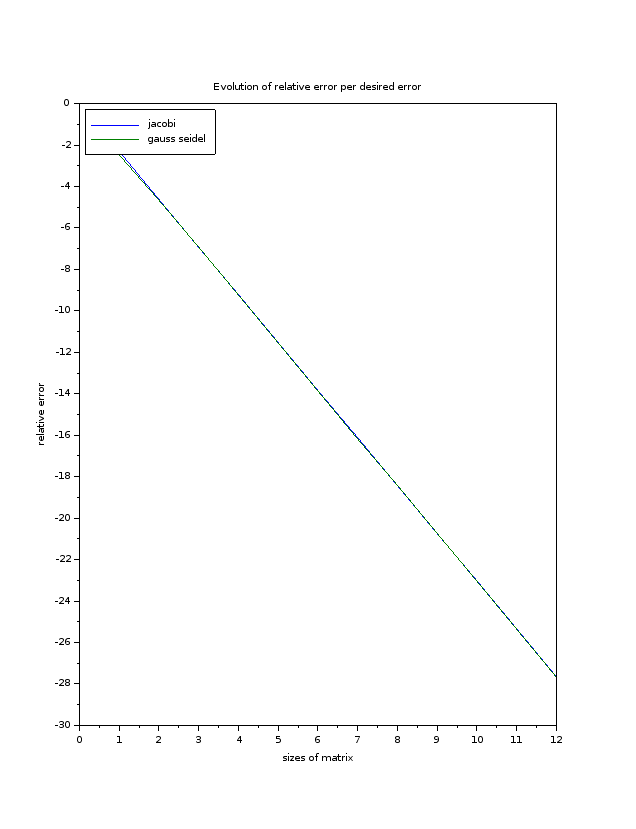
\includegraphics[scale=0.5]{img/error_relres.png}

Ici ce n'a pas vraimment grand intéret de calculer l'erreur relative
car justement on varie l'erreur souhaité et donc on y ariive à un
moment. Plus on baisse l'erreur souhaité plus l'erreur relative est faible.

\subsubsection{Conclusion}

Ces 2 graphiques confirmes que la méthode de Gauss Seidel converge
plus rapidement que celle de Jacobi en termes de nombre d'itération de
la méthode. Mais cela ne veut pas dire qu'elle est plus rapide.

\subsection{Question 5}

Nous prenons un $n = 10$ et une erreur souhaité de $e = 10^{-8}$ pour
le problème de poisson 1D et nous allons étudier sa convergence :

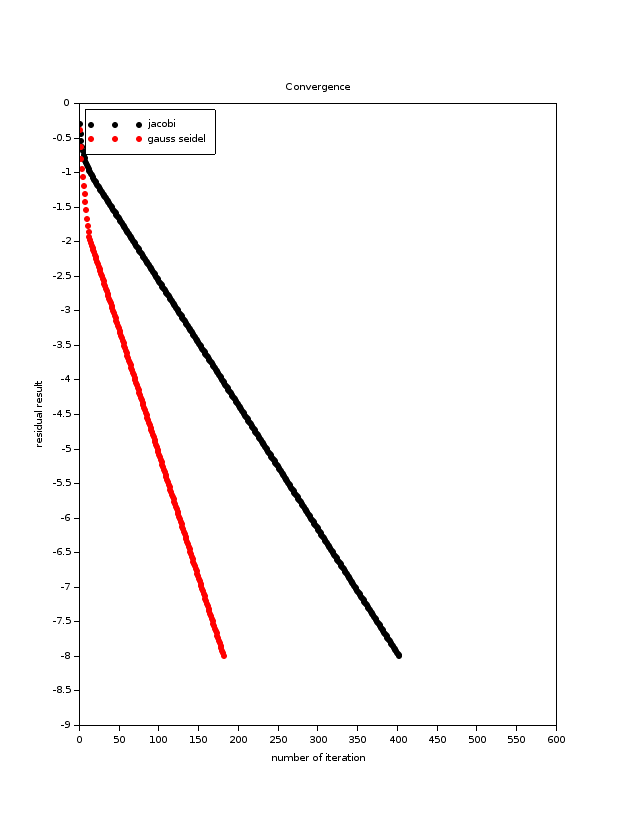
\includegraphics[scale=0.5]{img/convergence.png}

On voit que pour les 2 méthodes il y a convergence à $10^(-8)$ pour
notre problème. Et que le nombre d'itération de Jacobi est 2 fosi plus
élevé que celui de Gauss Seidel

\section{Exercice 7}

\subsection{Question 1}

Soit $$x^{k + 1} = x^k + \alpha (b - Ax^k)$$
avec $\alpha \in \mathbb{R}^{*+}, A \in \mathbb{R}^{n \cdot n}, b, x^k
\in \mathbb{R}^n, k \in \mathbb{N}$\newline

\begin{equation*}
  \begin{split}
    x^{k+1} & = x^k + \alpha b - \alpha A x^k \\
    & = (I - \alpha A) x^k + \alpha b \\
    & = G_{\alpha} x^k + \alpha b \\
  \end{split}
\end{equation*}

On pose $G_{\alpha} = I - \alpha A$\newline
\vspace{5mm}
$G_{\alpha}$ est inversible et l'équation ci-dessus converge si
$\rho(G_{\alpha}) < 1$

\subsection{Question 2}

Encadrement pour les valeurs propres (vp) de $G_{\alpha}$ qu'on note
$\mu_i$.\newline

\vspace{5mm}

Soit les vp réelles de A, noté $\lambda_i$ telles que :
$$ \lambda_{min} \le \lambda_i \le \lambda_{max} $$

Alors les vp de $G_{\alpha} = (I - \alpha A)$ sont telles  que
$$ 1 - \alpha \lambda_{max} \le \mu_i \le 1 - \alpha \lambda_{min}$$

\underline{Remarques :} Comment en ai-t-on arrivé à cette conclusion ?\newline

\vspace{5mm}

Soit $P^{-1}AP = D_A = \left[
  \begin{array}{ccc}
    \lambda_1 & ... & 0 \\
    ... & \lambda_i & ... \\
    0 & ... & \lambda_n \\
  \end{array}
  \right]$

\begin{equation*}
  \begin{split}
    P^{-1}G_{\alpha}P & = I - \alpha D_A \\
    & = D_{G_{\alpha}} \\
    & = \left[
      \begin{array}{ccc}
        1 - \alpha \lambda_1 & ... & 0 \\
        ... & 1 - \alpha \lambda_i & ... \\
        0 & ... & 1 - \alpha \lambda_n \\
      \end{array}
      \right]
  \end{split}
\end{equation*}

Ce qui implique que $\mu_i = 1 - \alpha \lambda_i$\newline

\vspace{5mm}

Et comme

\begin{gather*}
    \lambda_{min} \le \lambda_i \le \lambda_{max} \\
    - \alpha \lambda_{max} \le - \alpha \lambda_i \le - \alpha
    \lambda_{min} \\
    1 - \alpha \lambda_{max} \le 1 - \alpha \lambda_i \le 1 - \alpha
    \lambda_{min} \\
\end{gather*}

\subsection{Question 3}

Quelle condition sur $\alpha$ pour que Richardson converge ?\newline

\vspace{5mm}

Les différentes conditions proviennent du signe des valeurs propres de
A.

\begin{itemize}
\item Soit $\lambda_{min} < 0$ et $\lambda_{max} > 0$\newline
  alors au moins une valeur propre de $\mu_i$ est $> 1$\newline
  car $1 - \alpha \lambda_{max} < 1$ et $1 - \alpha \lambda_{min} > 1$\newline
  Donc $\rho(G_{\alpha}) > 1 =>$ Diverge \newline
  \underline{Remarque :} cela marche uniquement pour les matrices
  défini positives
\item $\lambda_{min} > 0$ toutes les vp de A sont positives\newline
  \underline{Remarque :} cas des matrices SPD\newline
  Alors la convergeance garantie par $\rho(G_{\alpha}) < 1$, est
  satisfaite pour :
  $$ 1 - \alpha \lambda_{min} < 1 => \alpha > 0 $$
  $$ 1 - \alpha \lambda_{max} > -1 => \alpha <
  \frac{2}{\lambda_{max}} $$
  Donc la méthode converge pour
  $$ 0 < \alpha < \frac{2}{\lambda_{max}} $$
\end{itemize}

\subsection{Question 4}

Essayons maintenant de déterminé la valeur optimale de $\alpha$ que
l'on notera $\alpha_{opt}$.\newline

\vspace{5mm}

Tout d'abord quelle est la caractéristique du $\alpha_{opt}$. C'est la
valeur de $\alpha$ qui minimise $\rho(G_{\alpha})$.\newline

\vspace{5mm}

Donc $ \rho(G_{\alpha}) = max\{|1 - \alpha \lambda_{min}|, |1 - \alpha
\lambda_{max}|\} $\newline

\vspace{5mm}

On trace les fonctions :

\begin{equation*}
  \begin{split}
    f_{min, max} : \mathbb{R} & \rightarrow
    \mathbb{R}\\
    \alpha & \rightarrow | 1 - \alpha
    \lambda_{min, max} | \\
  \end{split}
\end{equation*}

Intersection entre $-1 + \alpha \lambda_{max}$ et $1 - \alpha
\lambda_{min}$ \newline

\vspace{5mm}

Donc,

$$ -1 + \alpha_{opt} \lambda_{max} = 1 - \alpha_{opt} \lambda_{min} $$
$$ \alpha_{opt} = \frac{2}{\lambda_{min} + \lambda_{max}} $$

\subsection{Question 5}

\begin{algorithm} [H]
  \SetAlgoLined
  \KwData{$A \in \mathbb{R}^{n \cdot n}$, $b \in \mathbb{R}^{n}$,
    $max\_count, \epsilon, \alpha \in \mathbb{R}$}
  \KwResult{$x \in \mathbb{R}^{n}$, $count, relres \in \mathbb{R}$, $resvec \in
    \mathbb{R}^{n}$}

  count = 0 \Comment{Initialisation du compteur}

  x = zeros(n) \Comment{Init. vecteur résultat à 0}

  normb = norm(b) \Comment{Init. norme de b}
  
  r = b - A * x \Comment{Initialisation du résidu}

  relres = norm(r) / normb \Comment{Init. erreur relative}
  
  \While{$relres > \epsilon$ and $count < max\_count$}{

    x = x + $\alpha$ * r     \Comment{Calcul de richardson}
    
    r = b - A * x \Comment{Calcul du résidu}

    
    relres = norm(r) / normb \Comment{Calcul de l'erreur relative}
    
    resvec(count) = relres \Comment{Sauv. vecteur}


    count = count + 1     \Comment{Incrémentation du compteur}
  }

  \caption{Méthode de Richardson}
\end{algorithm}

\vspace{5mm}

\underline{Complexité :}

\begin{itemize}
\item en temps : indéterminé
\item en temps pour une itération : $O(n^2 + 3n)$ (1 produit
  \textbf{matrice x vecteur}, 1 produit \textbf{scalaire x vecteur} et
  2 addition/soustraction \textbf{vecteur x vecteur})
\item en espace : $O(n^2 + 3n)$ (1 matrice et 3 vecteur)
\end{itemize}

\section{Annexe}

Dépôt github : \url{https://github.com/Sholde/CN/tree/master/partie_2/poisson}

\end{document}
